% !TEX root = ../../main.tex

\chapter{Introduction}
\label{chapter:introduction}

The field of Machine Learning (ML) has gained massive traction over the last few decades, with both industry and academia investing substantial efforts to enhance data availability and the performance of ML algorithms. This performance factor encompasses both the accuracy of a model, and the computational and time costs associated with training these models.  To make training more efficient, researchers have proposed a novel approach called factorized learning \cite{orion_learning_gen_lin_models}. This approach enables models to be trained on normalized data, opening up new possibilities for more efficient model training. Factorized learning is applicable to a wide range of realistic ML workflow scenarios and joinable data sources.

\begin{figure}[h]
    \centering
    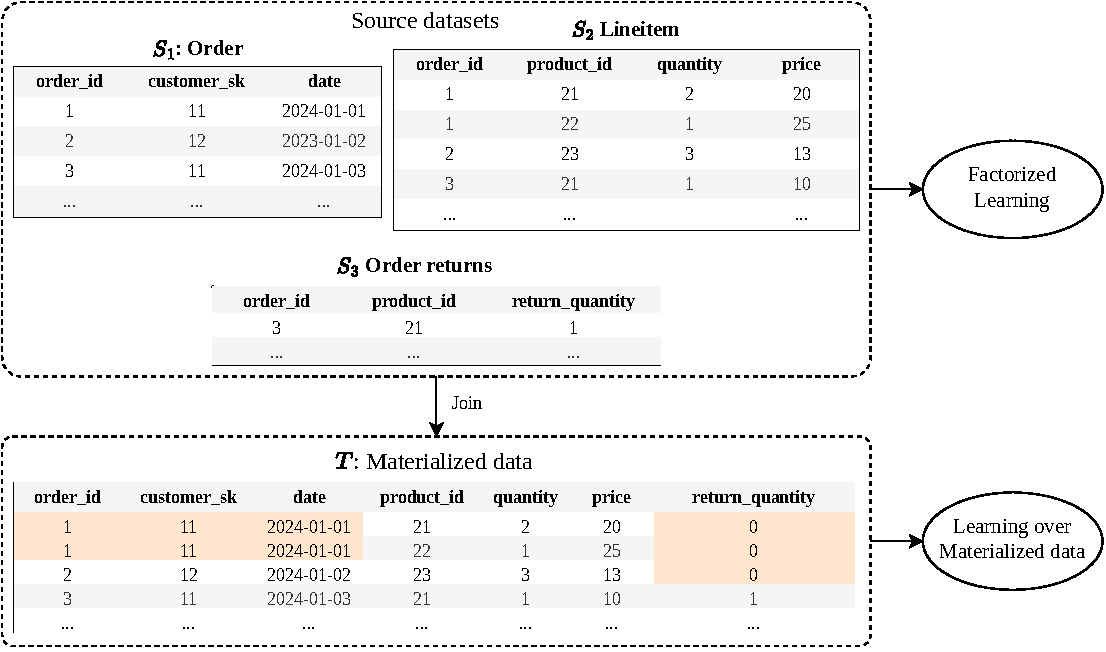
\includegraphics[width=0.95\linewidth]{chapters/01_introduction/figures/running-example-intro.pdf}
    \caption[Running Example: Source tables $S$ and target table $T$]{\textbf{Running Example: Source tables $S$ and target table $T$}. \\ Illustration of input data used for factorized Learning vs. Learning over Materialized data, schema from TPCx-AI \cite{tpcx-ai} use case 1 (unused columns not shown). Target redundancy avoided by factorization shown in orange.}
    \label{fig:running-example-fac-vs-mat}
\end{figure}

In a typical machine learning scenario, the first step for a data scientist aiming to train a model is gathering the necessary data for the training process. Often this data comes from disparate sources. Therefore, they first need to join these sources to create a single dataset to use as input for an ML model. This is achieved through a process called Data Integration (DI). The act of executing the join between these tables is called materialization \cite{rel_db_glossary}. Factorized learning eliminates this prerequisite to the training process by learning directly from the source datasets, without first joining them. \autoref{fig:running-example-fac-vs-mat} illustrates the difference between factorized learning and learning over materialized data. The reason factorized learning can be more efficient is that the values in the materialized data (orange cells in $T$ in the figure) do not lead to redundant computations during training. However, the source datasets can also have redundant values, and this redundancy is not the only factor that affects the efficiency of factorized learning. Apart from the data-characteristics (which include redundancy), model parameters and hardware characteristics can also influence the choice between factorized learning and materialization.

Thus, because factorization does not always increase efficiency, there is a need to be able to pick out those cases where factorization is beneficial. This decision between factorization and materialization is a multidimensional cost optimization problem. It is an interesting and important problem because factorized learning is a very novel approach to the fundamentals of machine learning. It has the potential to reduce the cost of model training without affecting performance. Factorized ML could also be easily extensible to federated learning in a scenario where computations involving a source dataset are executed in the silo in which the dataset is located \cite{amalur}.

However, solving this problem is challenging because the optimization space is exceptionally large and may be hardware dependent. Previous solutions, such as Morpheus \cite{morpheus} and Amalur's cost estimation \cite{schijndel_cost_estimation}, have focused on theoretical cost or simple heuristics without considering the hardware dimension.

\begin{figure}[h]
    \centering
    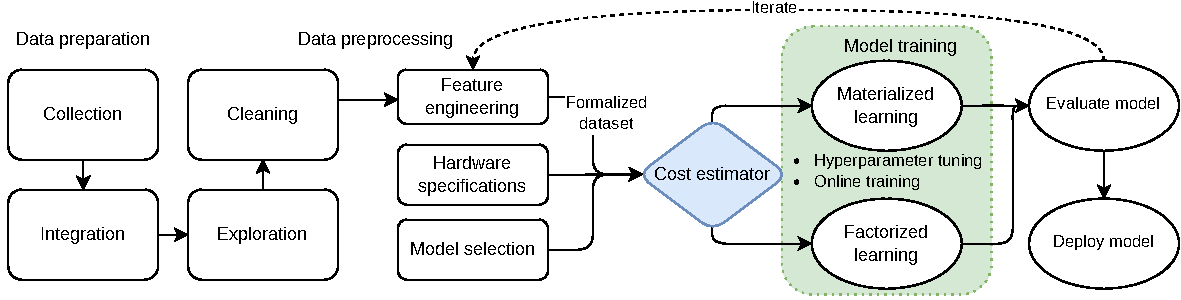
\includegraphics[width=0.95\linewidth]{chapters/01_introduction/figures/ML-Pipeline.pdf}
    \caption{Function of this thesis' cost model in an ML pipeline.}
    \label{fig:ml-pipeline}
\end{figure}

\autoref{fig:ml-pipeline} shows the applicability of the cost model we propose. For an ML practitioner aiming to optimize their training processes with the use of factorized learning, the data preparation and preprocessing steps do not change. The need to gather source datasets and define how to e.g., join and clean them does not change. After finishing pre-processing, formalizing how the datasets should be joined, and having decided what model they want to train, the cost model predicts the optimal training method. Using such a cost model to decide whether to materialize or factorize can result in considerable time savings. Particularly in scenarios where the total training time is high,  such as hyperparameter tuning or training complex models. This is shown in \autoref{sec:5-motivation}.

\section{Research Questions \& Contributions}
This thesis focuses on facilitating the adoption of factorized machine learning by developing a model that can accurately decide the optimal approach (from factorized and materialized computation) for training a machine learning model, considering the data, model, and hardware dimensions.

\subsection{Research Questions}
The research questions answered in this thesis are:
\begin{enumerate}[leftmargin=1.5cm, label=\emph{RQ.\arabic*}]
    \item How can we optimize and implement Factorized Machine Learning for GPUs?
    \item How can we accurately predict the optimal choice between factorized or materialized training of a Machine Learning model, on CPU and GPU, through leveraging knowledge about model, data, and hardware characteristics?
\end{enumerate}

\subsection{Contributions}
The Research Questions are answered by providing the following contributions:
\begin{enumerate}[leftmargin=1.5cm, label=\emph{C.\arabic*}]
    \item A GPU optimized implementation of Amalur's Factorized Machine Learning framework.
    \item A cost model that predicts whether factorized or materialized learning is faster, capable of accurate predictions regardless of dataset, model hyperparameters, or hardware used. This cost model is the result of a detailed study that compares multiple cost calculation strategies.
\end{enumerate}

\section{Running Example}
Throughout this thesis we use a running example, based on TPCx-AI\cite{tpcx-ai} use case 1, to explain various concepts. The scenario is that of a data scientist working for an ecommerce firm, who is tasked with creating a data science pipeline to perform customer segmentation. Three tables are joined to create a single table, which is then used as input in a K-Means clustering model. The schema of the tables and the joined table are shown in \autoref{fig:running-example-fac-vs-mat}.

The three tables that need to be joined are the \textbf{Orders} table ($S_1$), the \textbf{Lineitem} table ($S_2$), and the \textbf{Order returns} table ($S_3$). The \textbf{Orders} table contains information about orders made by customers, the schema of this table is $S_1(order\_id$, $customer\_sk$, $\ date)$. The \textbf{Lineitem} table contains information about the items in each order, its schema is $S_2(order\_id$, $product\_id$, $quantity$,  $price)$. The \textbf{Order returns} table, having schema $S_3(order\_id$, $product\_id$, $return\_quantity)$, contains information about the returns made by customers.

The joined table contains all the columns from the three source tables, and is used as input for the K-Means clustering model. It is created by first left joining $S2$ with $S1$ on shared columns $order\_id$ and $product\_id$, then joining the result of this with $S1$ on $order\_id$. After this we have $T(order\_id$, $customer\_sk$, $date$, $product\_id$, $quantity$, $price$, $return\_quantity)$.

\section{Cost Estimation for Factorized Machine Learning}
To develop a cost model that can accurately predict whether factorized or materialized learning is faster for a given ML task, we capture the runtime of training types for a set of scenarios. We vary the data used, the models trained, and the hardware settings. These collected results are then used as training data to create several types of cost models.

Evaluation on real-world datasets show that our models outperform the state-of-the-art (SOTA), specifically the \textbf{Hybrid} model, which combines a Linear Regression and an XGBoost model, performs well. It outclasses the SOTA in scenarios with real-world datasets, reaching \textbf{80\%} of the maximum achievable time saved. This cost model also generalizes, only losing \textbf{18\%} of its predictive power in scenarios with novel hardware settings and datasets.

\section{Outline}
This section provides an overview of the structure of the remainder of this thesis. We start with the theoretical concepts and principles that underpin our study in \autoref{chapter:preliminary}. The literature review (\autoref{chapter:literature}) reviews existing research relevant to our topic and identifies gaps or limitations in the existing literature. In the methodology chapter (\autoref{chapter:methodology}), we describe our overall approach to this empirical study, including the breakdown and motivation of the independent variables chosen.  In \autoref{chapter:cost-estimation}, we detail the statistical and analytical methods used to analyze the data, present the results of each experiment, and include visualizations to illustrate key findings. Next, in \autoref{chapter:evaluation-discussion}, the results are evaluated and discussed. It starts with an explanation of how the empirical results were gathered, followed by a discussion of the results of the experiments in relation to the research questions. Here, we also evaluate the validity and reliability of the results and compare our findings with those of the existing literature. This chapter ends with an in-depth interpretation and discussion of the results and their implications.  Finally, in the conclusion chapter (\autoref{chapter:conclusion}), the main contributions and findings of this thesis are summarized, and we provide an outlook for future research.

